% !TEX root = ../Network.tex



\documentclass[class=article, crop=false]{standalone}
\usepackage[subpreambles=true]{standalone}
\usepackage{import}
\begin{document}










\subsection{Machines virtuelles - configuration réseau}

Les différents paramètres de configuration de la carte réseau de VirtualBox sont:
\begin{itemize}

\item \textbf{NAT} (Network Address Translation): l'accès au réseau se fait à partir de l'adresse IP de la machine hôte.
\begin{example}
Remarque: quand \textit{un réseau} fonctionne en NAT, chaque machine dans le réseau privé possède une adresse privée. Le routeur est le seul à avoir une adresse publique qu'il utilise pour communiquer sur le réseau public (internet).
\end{example}

\item \textbf{Accès par pont} (bridge): la machine virtuelle "invitée" (dans VirtualBox) passe par dessus la machine virtuelle "hôte" pour se connecter directement à la carte réseau de l'ordinateur et ainsi obtenir sa propre adresse IP.

\item \textbf{Réseau interne}: réseau virtuel isolé sur lequel les machines virtuelles communiquent entre elles. Les VM ne peuvent pas se connecter ni réseau extérieur, ni à l'hôte.

\item \textbf{Réseau privé hôte}: réseau interne dans lequel les machines virtuelles peuvent communiquer entre elles et avec la machine hôte mais pas avec l'extérieur.

\end{itemize}
Quelle configuration faut-il pour être \textbf{joignable de l'extérieur} ? \textit{Accès par pont.} \\
Quelle configuration utiliser pour \textbf{connecter 2 VM} exécutées sur le même ordinateur ? \textit{Réseau interne (?)} \\
Expliquer les \textbf{options de configuration} ci-dessous:
\begin{center}
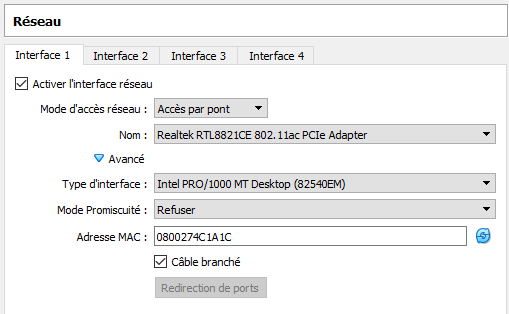
\includegraphics[width=0.65\textwidth]{images/Labo1ConfigurationReseau.png}
\end{center}
\begin{itemize}
\item \textbf{Nom}: carte réseau.
\item \textbf{Type d'interface}: pilote informatique (driver) - programme permettant la communication entre l'OS et un périphérique (ici, la carte réseau).
\item \textbf{Mode Promiscuité}: configuration de la carte réseau, qui permet à celle-ci d'accepter tous les paquets qu'elle reçoit, même si ceux-ci ne lui sont pas adressés.
\item \textbf{Adresse MAC}: aussi appelée \textit{adresse physique}, est un identifiant physique unique au monde stocké dans une carte réseau.
\item \textbf{Câble branché}: utile pour simuler qu'aucun câble n'est branché à cette interface. Si la case est décochée, la VM ne sera plus joignable.
\item \textbf{Redirection de ports}: idk.
\end{itemize}










\subsection{Paramètres d'un réseau hôte}

\begin{itemize}
    \item \textbf{Adresse IP statique}: adresse logique IP (V4) fixe, répartie sur 4 octets.
    \item \textbf{Masque de sous réseau}: masque distinguant les bits d'une adresse IPv4 utilisés pour identifier le sous-réseau de ceux utilisés pour identifier l'hôte.
\begin{example}
Exemple:
\begin{itemize}
    \item adresse réseau: 192.57.194.0
    \item adresse hôte: 192.57.194.12
    \item masque de sous-réseau: 255.255.255.0
\end{itemize}
\end{example}
\item \textbf{Adresse IP dynamique}: adresse IP reçue dynamiquement via un serveur extérieur et renouvelée à intervalles réguliers.
\item \textbf{Adresses IP supplémentaires}: adresses IP utilisées en plus de celle de base.
\item \textbf{Serveur DNS}: serveur qui permet de faire le lien entre adresse IP et FQDN (Fully Qualified Domain Name).
\begin{example}
Exemple:
\begin{itemize}
    \item Domaine du site internet: google.com
    \item Adresse IP du domaine: 216.58.204.110
\end{itemize}
\end{example}
\item \textbf{Host Name}: nom d'hôte Local d'une machine et/ou nom d’hôte DNS.
\item \textbf{Passerelle par défaut}: adresse de l’élément qui va permettre la discussion entre deux hôtes, par exemple un routeur, serveur ou une boxe internet. Équivalent d'un panneau "toutes directions", vers lequel sont dirigés les paquets dont le chemin vers la destination est inconnu.
\item \textbf{Passerelles supplémentaires}: passerelles correspondant au chemin vers des réseaux connus.
\item \textbf{Firewall}: dispositif qui autorise/interdit le trafic réseau sur base de certains critères.
\item \textbf{Carte réseau}: périphérique permettant de connecter son ordinateur à un réseau. \\
Propriétés:
\begin{itemize}
    \item \textbf{Mac Address}: adresse matérielle d'une interface Ethernet. Sur 48 bits, notée en hexadécimal. La première partie correspond au constructeur.
    \item \textbf{Duplex}: canal de communication qui transporte l'information dans les deux sens (bidirectionnel). Un canal qui transporte l'information dans un seul sens est appelé simplex (monodirectionnel).
    \begin{itemize}
        \item \textbf{Full-duplex}: l'information peut être transportée simultanément dans les deux sens.
        \item \textbf{Half-duplex}: l'information est transportée dans un sens à la fois (comme des talkie-walkies).
    \end{itemize}
    \item \textbf{Débit}: nombre maximal de b/secondes qui peuvent circuler par une interface.
\end{itemize}
Remarque: b/seconde = bits/seconde, alors que: B/seconde = bytes/seconde (byte = octet).
\end{itemize}










\subsection{Liste d'enregistrements DNS}

\begin{center}
\begin{tabular}{|c|c|c|} \hline
Enregistrement & Signification du nom & Fonction \\ \hline
A & Adresse IPv4 & nom de domaine $ \implies $ IPv4 \\
AAAA & Adresse IPv6 (4$\times$ la taille d'une IPv4) & nom de domaine $ \implies $ IPv6 \\
CNAME & Nom Canonique & nom de domaine $ \implies $ nom de domaine \\
MX & Mail Exchanger & nom de domaine $ \implies $ liste de serveurs (= hôtes) \\ \hline
\end{tabular}
\end{center}

Exemples:
\begin{itemize}
    \item Type A: \texttt{www.example.com} $ \rightarrow $ \texttt{192.168.1.32}
    \item Type AAAA: \texttt{www.example.com} $ \rightarrow $ \texttt{2a02:a03f:417b:3300:3c88:a5ee:451b:82ca}
    \item Type CNAME: \texttt{www.hotmail.com} $ \rightarrow $ \texttt{www.outlook.com}
    \item Type MX:
    \begin{itemize}
        \item mail: \texttt{greg@example.com}
        \item nom de domaine: \texttt{example.com}
        \item hôtes: \texttt{server1.example.com}, \texttt{serveur2.example.com}, etc.
    \end{itemize}
\end{itemize}

Remarque: les hôtes dans les enregistrements de types MX \textit{doivent} aussi avoir un enregistrement de type A (ou AAAA) sur le même serveur DNS (pas de CNAME).










\subsection{Serveur FTP/TFTP}

\begin{itemize}
\item \textbf{Serveur FTP} (File Transfer Protocol): \\
Protocole de partage de fichiers \textit{en clair}, sur un réseau TCP/IP. L'authentification est requise mais peut aussi être anonyme (si le serveur l'autorise). On utilise FTPS pour une transmission sécurisée.
\item \textbf{Serveur TFTP} (Trivial File Transfer Protocol): \\
Protocole \textit{simplifié} de transfert de fichiers, fonctionne en UDP. Il est souvent utilisé dans les systèmes de démarrage PXE), les configurations d'équipement de réseau, d'importation/exportation, etc.
\end{itemize}





\end{document}
